\documentclass{article}
\usepackage[T1]{fontenc}
\usepackage{lmodern}
\usepackage{graphicx}
\usepackage{amsmath,amssymb}
\usepackage[a4paper,margin=2cm]{geometry}
\usepackage[absolute,overlay]{textpos}
\setlength{\TPHorizModule}{1mm}
\setlength{\TPVertModule}{1mm}
\usepackage[indonesian]{babel}
\usepackage{hyperref}
\setlength{\emergencystretch}{2em}
% unit: Halaman 6

\begin{document}

% === Halaman 6 (llm) ===

\vspace{92.07mm}

\vspace{10mm}
\textbf{Gambar 1 Skema global algoritma DES}

% deskripsi: Diagram alir skema global algoritma DES yang menunjukkan proses dari blok plainteks melalui Initial Permutation (IP), proses Enciphering yang diulang 16 kali dengan sub-key $K_i$, hingga Final Permutation ($IP^{-1}$) menjadi blok cipherteks, serta proses Key expansion dari kunci $K$.
% bbox normalisasi: [0.2800, 0.5000, 0.8900, 0.8100]
\begin{textblock*}{128.10mm}(58.80mm,148.50mm)
\noindent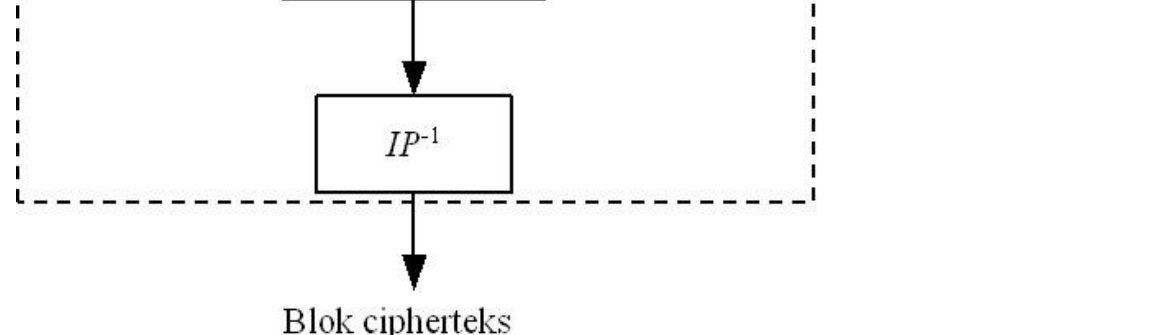
\includegraphics[width=128.10mm,height=92.07mm]{../../images/llm/page_006_img_01.png}%
\end{textblock*}

\end{document}
